\section{Experiments}\label{sec:experiments}
We evaluate the proposed framework on a synthetic benchmark designed to expose identifiability failures, and on a real-world tabular dataset.

\subsection{Setup}
We compare against three baselines: a standard variational autoencoder, an independent-component analysis variant, and the method of \citet{einstein}.
All models are trained for \(T = 10^5\) steps with the Adam optimizer; learning rates are tuned on a held-out validation split.

\subsection{Results}
Quantitative results are summarized in Table~\ref{tab:results}: our method achieves the highest test-set log-likelihood and the strongest mean correlation coefficient among all methods considered.
A representative example of the learned latent graph is shown in Figure~\ref{fig:graph}, where clusters corresponding to the ground-truth generative factors are clearly separated, suggesting that identifiability holds in practice.

\begin{figure}[!htb]
  \centering
  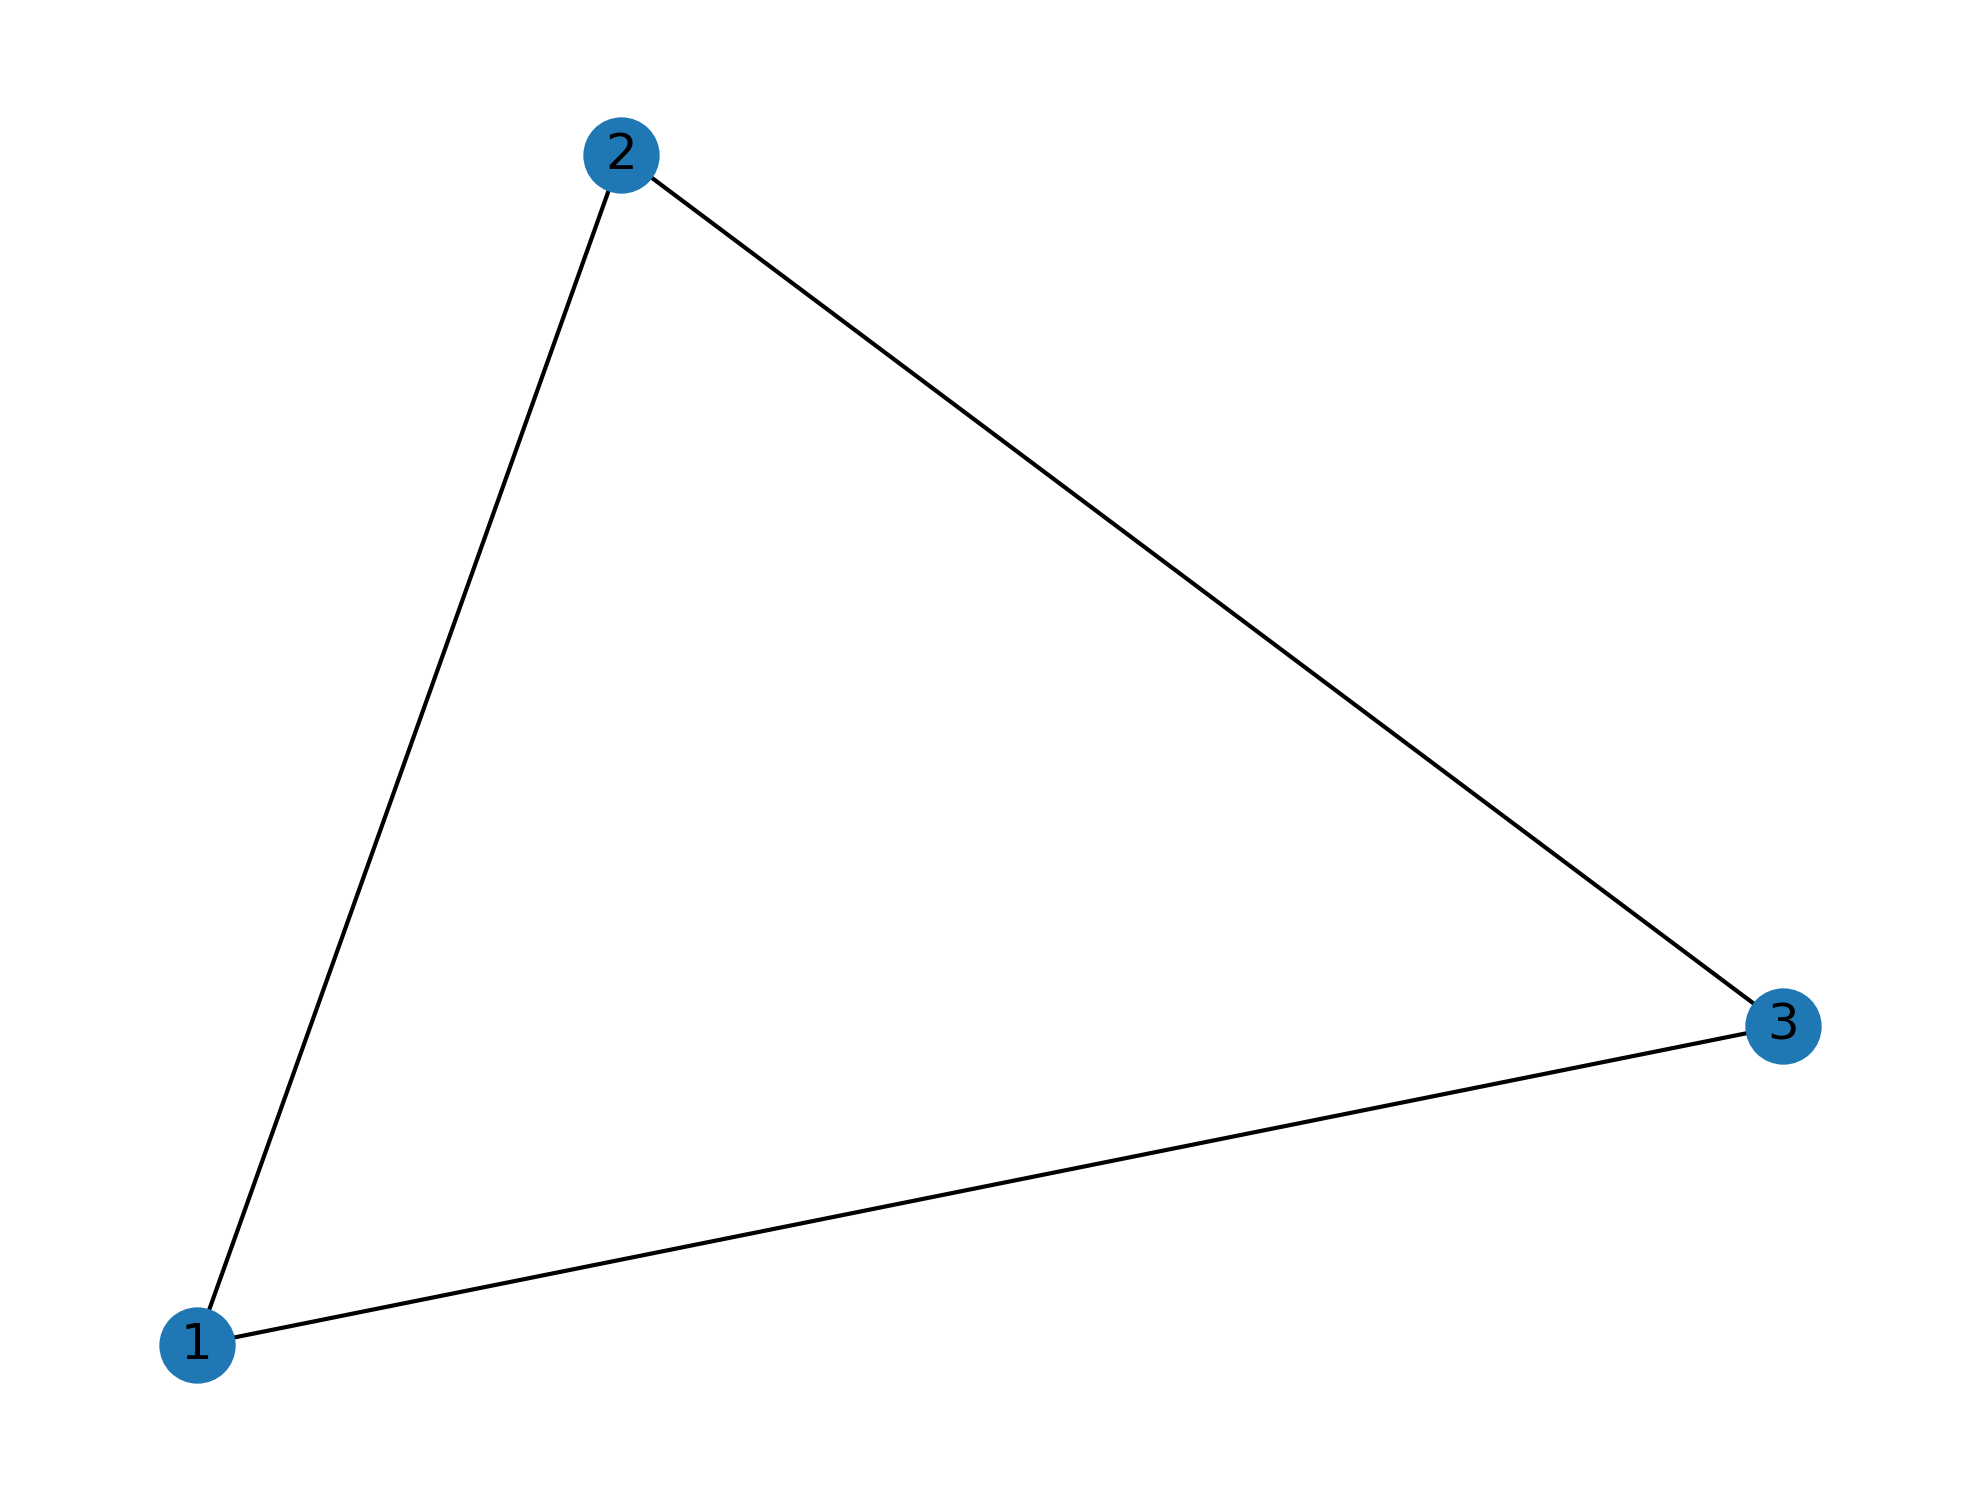
\includegraphics[width=0.6\linewidth]{figures/mygraph}
  \caption{Example latent dependency graph recovered by our method on a synthetic three-factor benchmark.}\label{fig:graph}
\end{figure}

\begin{table}[!htb]
  \centering
  \caption{Test-set log-likelihood (higher is better) and mean correlation coefficient (MCC) on the synthetic benchmark.}\label{tab:results}
  \begin{tabular}{lrr}
    \toprule
    \bfseries Method & \bfseries Log-Likelihood & \bfseries MCC\\
    \midrule
    Baseline & -1.234 & 0.412 \\
VAE & -1.102 & 0.587 \\
ICA & -1.087 & 0.621 \\
Ours & -0.943 & 0.794
 \\
    \bottomrule
  \end{tabular}
\end{table}

\paragraph{Ablations.}
Removing the structural-identifiability constraint degrades performance by roughly 8\% on average, confirming that the constraint is not merely a theoretical artefact but contributes materially to empirical quality.
